The text about entire system stuff and more stuff


\begin{figure}[htb]
	\centering
	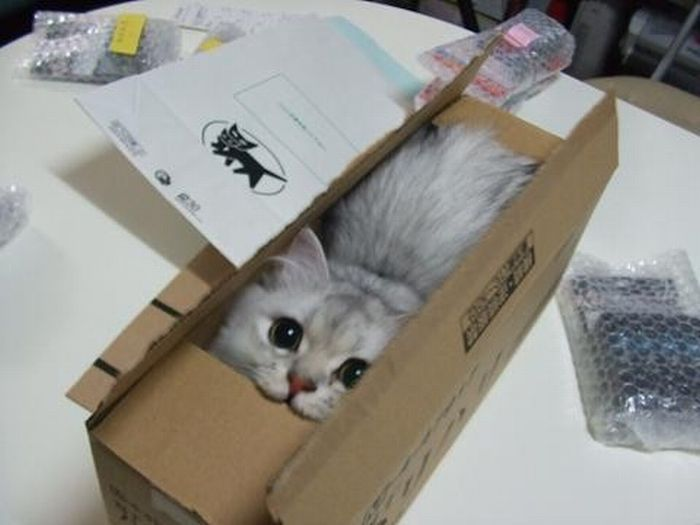
\includegraphics[width=\linewidth]{images/boxcat.jpg}
	\caption[Overview of the entire system]{\textit{System overview.}}
	\label{fig:system_overview}  %Skapar referens till figuren
\end{figure}

\subsection{Config file system}
The system configuration file contains all image processing pipeline parameters together with the address of the current destination web service, where counting results are to be presented.

\subsection{Network module}
The network module manages all system input/output. Currently, support exists for all OpenCV-compatible RGB cameras as well as the Microsoft Kinect depth sensor. The module is designed to be as modular as possible, allowing for a relatively easy replacement integration of new sensor types. Support also exists for running several sensors in parallel. Communication with the web server also takes place here.

\subsection{Algorithm Interface}
Algorithm interfaces and stuff

\subsection{Debug and Config GUI}
short about config gui
